\documentclass[11pt]{article}
\usepackage[margin=1in]{geometry}
\usepackage{graphicx}
\usepackage{amsmath,amssymb}
\usepackage{booktabs}
\usepackage{xcolor}
\usepackage{listings}
\usepackage[colorlinks=true,linkcolor=blue,citecolor=blue,urlcolor=blue]{hyperref}
\usepackage{enumitem}

\lstset{basicstyle=\ttfamily\footnotesize,breaklines=true,frame=single,
        backgroundcolor=\color{gray!8},columns=fullflexible}
\newcommand{\code}[1]{\texttt{#1}}

\title{\textbf{Provenance-Certified KKR Convergence Assistance:\\
\texttt{ml\_assist}, PotentialBank~v1, and Same-Structure Warm Starts}\\[3pt]
\large An AiiDA-native early-abort framework and a certified potential-reuse bank ---\\
with a live pilot, a held-out benchmark, and explicitly benchmarked limits}
\author{%
% TODO before submission: fill author full name(s), affiliation, email, ORCID.
M.~R.~Hemmati\thanks{TODO: affiliation; email; ORCID --- to be filled before CPC submission}%
% \and Co-author name\thanks{affiliation}
}
\date{2026-08-13}

\begin{document}
\maketitle

\begin{abstract}
\noindent
Self-consistent-field (SCF) convergence is the practical bottleneck of KKR and Bogoliubov--de~Gennes
(BdG) Green's-function DFT campaigns: many runs stall or diverge, wasting cluster time. We present an
\textbf{AiiDA-native convergence-control framework}, \code{ml\_assist}, that scores a run's first ten SCF
iterations and can abort doomed runs early --- an opt-in layer with a zero-risk default. The framework
ships a \textbf{frozen \code{numpy} random-forest scorer} (the AiiDA daemon has no scikit-learn) alongside
a \textbf{simple RMS-at-iteration-10 baseline}, both wrapped in a \textbf{per-cohort conformal early-abort
policy} that controls the false-abort rate after per-cohort calibration under calibration/test
exchangeability, with Mondrian per-stratum thresholds for conditional coverage.
A \textbf{live Fe-doped NbSe$_2$ pilot validates the abort machinery end-to-end}: a true early abort saved
$\sim$130 SCF iterations against its diverging counterfactual, and a would-be false abort on a
slowly-converging run was correctly withheld ($N{=}5$, descriptive). On a \textbf{336-run, leakage-clean
held-out replay with per-run convergence-target (\code{QBOUND}) labels}, the learned model does
\emph{not} beat the RMS@10 baseline on the primary NbSe$_2$ normal-state cohort (held-out AUC $0.83$
vs.\ $0.90$), \emph{does not transfer across materials} (other-material AUC $\approx$ chance), and a
NbSe$_2$-seeded conformal threshold does not transport (realized false-abort $0.47$) --- though
\textbf{per-cohort recalibration restores} realized $\approx$ target $\alpha$. We conclude that
\emph{reliable deployment requires per-cohort calibration and strong simple baselines}; the honest,
provenance-tracked framework --- not model superiority --- is the contribution.
We then present \textbf{PotentialBank~v1}, a provenance-certified extension of AiiDA-KKR that realizes the
warm-start lever: it retrieves, certifies, and reuses compatible \emph{same-structure} converged potentials.
AiiDA-KKR already provides the restart and \code{potential\_overwrite} primitives; our contribution is the
\textbf{certification and retrieval layer above them} --- byte-exact potential integrity (three-way SHA-256),
exact $Z$-sequence\,/\,NATYP compatibility, non-CPA\,/\,non-BdG scope control, and no guessed mapping.
PotentialBank~v1 is frozen at \textbf{237 unique certified donors (238 nodes)} across \textbf{8 material
families} and \textbf{33 F2-eligible materials}, with same-structure warm starts cutting SCF iterations
substantially (per-family, mixing- and contour-qualified). We claim \emph{no cross-material transfer and no
guaranteed acceleration}: donors reuse the identical structure, and nine hard cases are documented with root
causes. Separately, an engineering
effort repaired four cell-inappropriate BdG-workchain defaults, enabling the first end-to-end multi-atom
BdG run and its memory-scaling number. Everything ships as an installable \code{aiida-kkr-mlassist}
extension (with an optional convergence advisor), unit tests, and pre-registered success gates.
\end{abstract}

\paragraph{Keywords.} KKR Green-function DFT; SCF convergence; AiiDA provenance; potential reuse / warm start;
conformal prediction; reproducible workflows; certified donor potentials.

\begin{center}\small
\fbox{\parbox{0.97\linewidth}{
\textbf{Program summary}\\[2pt]
\emph{Program title:} \code{aiida-kkr-mlassist} / KKR Convergence Advisor / PotentialBank~v1.\\
\emph{Developer's repository:} \texttt{https://github.com/MRHemmati/kkr\_ml\_tools} (CPC library link and DOI
assigned on acceptance).\\
\emph{Licensing provisions:} MIT (open source).\\
\emph{Programming language:} Python (pure-\code{numpy} runtime core; AiiDA\,/\,\code{aiida-kkr} used only for
submission).\\
\emph{Nature of problem:} KKR SCF convergence wastes HPC time when runs stall or diverge; restarting from a
converged potential is standard and AiiDA-KKR provides the primitives, but choosing a \emph{compatible,
provenance-safe} donor is error-prone and unaudited.\\
\emph{Solution method:} an AiiDA-native, opt-in \code{ml\_assist} early-abort wrapper (pure-\code{numpy} scorer
+ RMS@10 baseline under a per-cohort conformal policy) and \textbf{PotentialBank~v1}, a provenance-graph donor
catalog admitting potentials only under strict E1 certification --- byte-exact SHA-256 integrity, exact
$Z$-sequence\,/\,NATYP compatibility, non-CPA\,/\,non-BdG scope, and no guessed mapping --- with an optional
same-structure warm-start advisor.\\
\emph{Restrictions:} normal-state, non-CPA for PotentialBank~v1; CPA\,/\,BdG and cross-material prediction are
not supported; warm-start reuse is same-structure only, with no guaranteed acceleration; raw potentials remain
in the AiiDA repository (referenced by SHA-256\,/\,provenance).\\
\emph{Unusual features:} strict provenance certification with byte-exact hashing, a no-guessed-mapping rule,
per-family same-structure warm-start benchmarks, and a documented catalog of hard cases.\\
\emph{Additional comments:} PotentialBank~v1 is frozen at 237 unique certified donors (238 nodes) across 8
families, 33 F2-eligible materials.
}}
\end{center}

\tableofcontents

\section{Goals and scope}
\label{sec:goals}
The parent project is a multi-year KKR / KKR-BdG superconductivity effort on 2H-NbSe$_2$ with
transition-metal dopants (V/Mn/Fe/Co), plus a Bi/NbBi subset. SCF convergence is the practical
bottleneck: many runs stall, diverge, or converge slowly, wasting cluster time. \code{ml\_assist} targets
three \emph{acceleration levers}:
\begin{description}[leftmargin=1.6em,itemsep=1pt]
  \item[L1 --- early abort] stop runs that are predicted not to converge, recovering their wasted tail.
  \item[L2 --- probe-and-commit mixing] race a few mixing settings briefly, commit the best.
  \item[L3 --- warm start] reuse a converged potential to halve iterations.
\end{description}
This report is in three parts. \textbf{Part~1} (Secs.~\ref{sec:goals}--\ref{sec:pilot}) covers
\code{ml\_assist} --- the early-abort framework (L1), its conformal policy, the live pilot, and the
leakage-clean held-out replay. \textbf{Part~2} (Sec.~\ref{sec:potbank}) presents \textbf{PotentialBank~v1},
the realized warm-start lever (L3): a certified catalog of single-structure converged potentials with an
optional convergence advisor and measured same-structure savings. \textbf{Part~3} (Sec.~\ref{sec:status}
onward) gives limitations and roadmap. The probe-and-commit mixing search (L2) reuses the same infrastructure
and remains estimated by the pre-registered campaigns.

\paragraph{Positioning.} KKR restart and potential reuse are \emph{not new}: AiiDA-KKR~\cite{aiidakkr} already
exposes the low-level primitives --- a KKR calculation can continue from a parent remote folder, automatically
extracting the converged potential, and the Voronoi step accepts an explicit \code{potential\_overwrite}. Our
contribution is the \textbf{layer above} these primitives. We introduce a provenance-certified extension of
AiiDA-KKR that systematically retrieves, validates, and reuses compatible \textbf{same-structure} donor
potentials for reproducible KKR warm starts, supplemented by an optional convergence advisor whose limits are
explicitly benchmarked. Concretely: a provenance-graph procedure discovers candidate donors; each is admitted
only under a strict eligibility policy (byte-exact potential integrity via a three-way SHA-256 match, exact
$Z$-sequence\,/\,NATYP compatibility, non-CPA and non-BdG scope control, and no guessed mapping); and the
resulting same-structure warm starts are benchmarked, with hard cases and negative results reported honestly.
This turns an available mechanism into an auditable, policy-controlled reuse system.

\paragraph{Design principles.} (1) \emph{Opt-in, zero-risk default}: absent an \code{ml\_assist} input the
workchain behaves identically to stock. (2) \emph{Advisory by default}; abort only when explicitly enabled
and the statistical guarantee is certifiable. (3) \emph{Per-system deployment}: we do not claim
cross-material transfer. (4) \emph{Honesty first}: negative results are reported as-is and are publishable.

\section{Background and tooling (what we used and why)}
\label{sec:tools}
\begin{description}[leftmargin=1.6em,itemsep=2pt]
  \item[JuKKR (KKRhost, voronoi, KKRimp).] The Green's-function DFT engine. SCF proceeds by iterating
  the potential; each iteration reports an RMS error and charge-neutrality. \emph{Why it matters for ML:}
  these per-iteration quantities are the raw signal from which convergence fate is predicted.
  \item[BdG extension.] Superconducting pairing is treated by doubling the Hamiltonian into
  Nambu (particle--hole) space; KKRhost-BdG additionally prints a pairing amplitude $\Delta$ per iteration.
  \emph{Why:} the pairing channel is a BdG-specific failure mode invisible to normal-state features.
  \item[AiiDA 2.7.] Workflow engine and provenance store. All calculations, inputs, and outputs are nodes
  in a directed provenance graph. \emph{Why:} it gave us a mineable corpus of historical runs \emph{and}
  is the natural place to deploy an opt-in wrapper workchain with full audit trail.
  \item[aiida-kkr.] The AiiDA plugin providing \code{kkr\_scf\_wc} (normal SCF) and \code{kkr\_bdg\_wc}
  (BdG chain). \emph{Why:} \code{ml\_assist} subclasses \code{kkr\_scf\_wc} to add the prediction hook.
  \item[scikit-learn (training only).] Random forests for the classifier. \emph{Why RF:} in distribution
  it beats logistic regression and the physical extrapolation heuristic and needs no feature scaling
  (Table~\ref{tab:baselines}). \emph{But out-of-sample} the strong baseline to beat is a plain
  RMS-at-iteration-10 rule, which the model does \emph{not} beat on the primary cohort
  (Sec.~\ref{sec:heldout}). \emph{Constraint:} scikit-learn is \emph{not} installed in the AiiDA daemon
  environment.
  \item[numpy (inference).] We export the trained forest to a flattened-array \code{.npz} and traverse it
  in pure \code{numpy}, reproducing scikit-learn's \code{predict\_proba} exactly. \emph{Why:} the daemon
  must score runs without scikit-learn; a numpy-only path removes that dependency (Sec.~\ref{sec:model}).
  \item[Conformal prediction.] A distribution-free wrapper that turns a score into a decision with a
  controlled error rate. \emph{Why:} it lets us \emph{control the false-abort rate} $\le\alpha$ after
  per-cohort calibration under calibration/test exchangeability, regardless of the model's calibration ---
  the safety property an abort policy needs (Sec.~\ref{sec:conformal}).
\end{description}

\section{Data and the provenance-mining audit}
\label{sec:data}
The AiiDA database holds $\sim$7{,}700 calculation nodes and $\sim$6{,}400 workchains (2021--2026). We
mined per-iteration RMS/charge-neutrality trajectories and outcomes. Three \emph{leakage-class}
corrections were essential and define the trustworthiness of every downstream number:
\begin{enumerate}[leftmargin=1.6em,itemsep=1pt]
  \item \textbf{Segment de-inflation.} Training rows were KKR \emph{segments} (up to 5 per workchain),
  not runs. Deduplicating to one cold-start row per run reduced 3{,}405 segments to \textbf{2{,}710 runs}
  (1{,}851 normal, 90\% converged).\footnote{Modeling uses the 1{,}830 normal runs with at least
  $T_{\mathrm{obs}}{+}2$ iterations (21 too-short runs excluded, needed to form the observation window);
  the BdG $\Delta$ study uses the 641 of 846 BdG runs whose \code{out\_kkr} was retrievable and parseable
  (Sec.~\ref{sec:delta}).}
  \item \textbf{Censoring scope.} 389 excepted/killed calculations are 100\% censored; the dataset is
  \emph{completed runs only}. Crashes/NaN-kills are out of scope and handled by a watchdog, not the model.
  \item \textbf{The Replay-OOF Invariant.} Any replay, preview, or ``deployment simulation'' number is
  out-of-sample or prospective \emph{by construction}, never in-sample. This was adopted after an in-sample
  shadow replay produced a spurious recall of $1.000$; the honest out-of-sample number is $0.70$
  (Sec.~\ref{sec:deploy}). The model that scores a run never trained on it (verified by node id).
\end{enumerate}
These corrections deflated some earlier claims (e.g.\ a cross-material transfer number collapsed from
$0.94$ to chance) --- an outcome we treat as a contribution, not an embarrassment.

\section{The convergence classifier}
\label{sec:model}

\begin{figure}[h]\centering
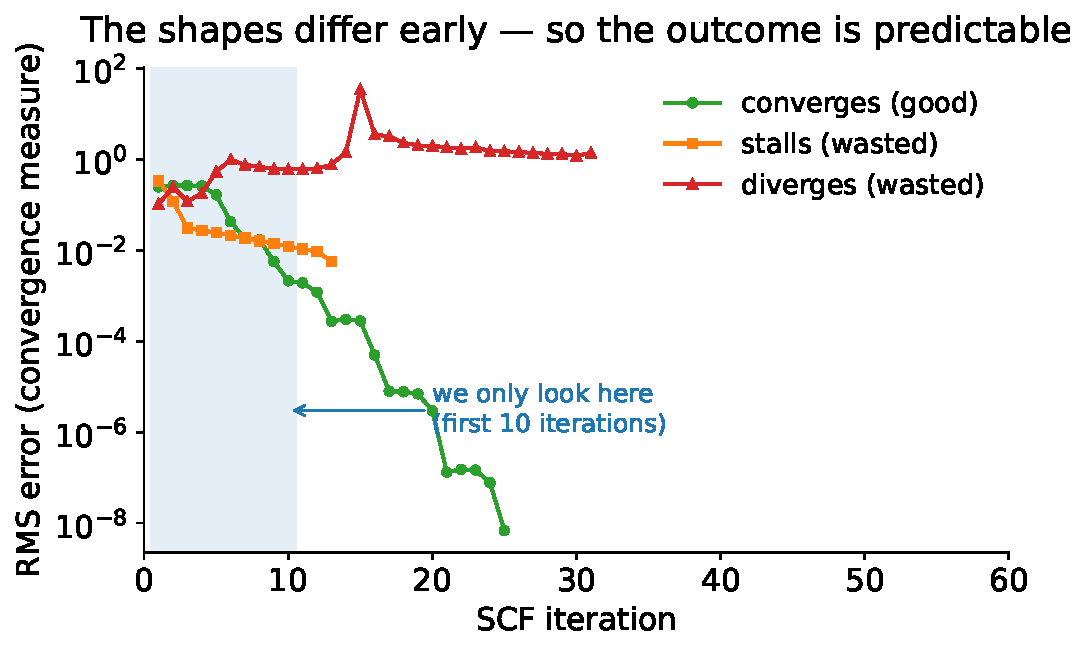
\includegraphics[width=0.72\textwidth]{figures/fig1_convergence_archetypes.pdf}
\caption{Why early prediction is possible. Converging, stalling, and diverging runs already trace
distinct shapes within the first ten iterations (shaded) --- the only data the model sees.}
\label{fig:archetypes}
\end{figure}

\paragraph{Features.} A 15-dimensional vector computed from the first $T_{\mathrm{obs}}=10$ iterations:
log-RMS window statistics (first, last, mean, std, min, drop, slope), two charge-neutrality statistics,
and three mixing parameters each with a missing-flag. A single canonical implementation is shared by
training and inference so they cannot drift (verified bit-identical).

\paragraph{Model and in-distribution accuracy.} A 400-tree balanced random forest. Its \emph{in-distribution}
5-fold cross-validation AUC is strong where data is plentiful and honestly weaker where it is thin
(Table~\ref{tab:permaterial}); the pooled normal-state 5-fold AUC is $0.944$. In distribution it beats
logistic regression and a physics extrapolation heuristic (Fig.~\ref{fig:auc}, Table~\ref{tab:baselines}).
\textbf{We deliberately do \emph{not} treat $0.944$ as the deployment headline}: it is a same-distribution
cross-validation number. The deployment-relevant question --- how the frozen model scores runs it has never
seen, against a simple RMS baseline --- is answered by the leakage-clean held-out benchmark of
Sec.~\ref{sec:heldout}, and there the model does \emph{not} beat RMS@10 and does \emph{not} transfer across
materials. The model is therefore deployed per-system with per-cohort calibration.

\begin{figure}[h]\centering
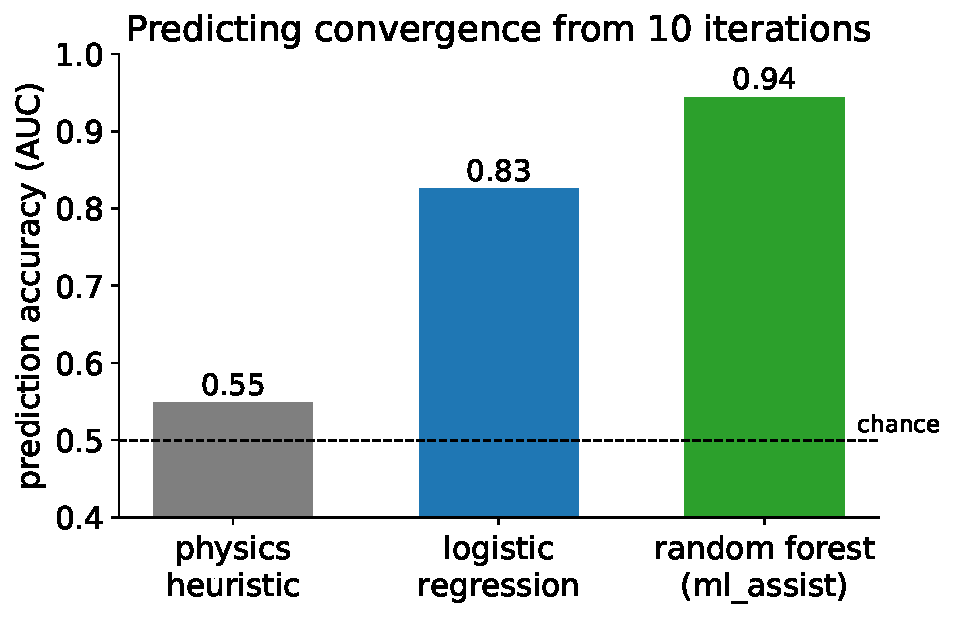
\includegraphics[width=0.56\textwidth]{figures/fig2_auc_baselines.pdf}
\caption{\emph{In-distribution only.} From ten iterations, the random forest cross-validates better than a
physics extrapolation heuristic or logistic regression (AUC; $0.5$ is a coin flip). This is \emph{not} the
deployment metric --- see the held-out benchmark (Fig.~\ref{fig:percohort}), where a simple RMS@10 rule
matches or beats the model out-of-sample.}
\label{fig:auc}
\end{figure}

\paragraph{A dropped complication (reported for the record).} A schedule-aligned observation window was
a pre-registered design lock intended to protect ``flat-start'' runs (flat, high-RMS early, then
converging). On the deduplicated data it gave \emph{no} measurable benefit: the fixed window already
separates flat-starters at AUC $\sim$0.90 (the discriminative signal is in charge-neutrality and mixing,
not the flat RMS slope). It was dropped for v1; the frozen model uses the plain fixed window.

\paragraph{Pure-\code{numpy} export and the float32 gotcha.} The forest is flattened to node arrays
(children, feature, threshold, per-leaf class probabilities) and traversed in \code{numpy}. Golden-parity
against scikit-learn is \textbf{exactly $0.0$}, verified running under the daemon interpreter (numpy 1.26,
no scikit-learn). One subtlety was decisive: scikit-learn casts inputs to \code{float32} for tree
traversal, so a \code{float64} comparison mis-routes samples sitting on a threshold tie (an initial
$10^{-2}$ parity failure). The numpy path compares in \code{float32}; embedded golden vectors (including
the exact edge sample that exposed the bug) guard against regression.

\section{The held-out benchmark: does the model beat a simple RMS rule?}
\label{sec:heldout}
The honest test of deployment value is a \emph{leakage-clean, out-of-sample} evaluation with correct
labels. We assembled \textbf{336 completed iffslurm runs verified absent from training} (by node id) and
scored each run's frozen first-ten-iteration features. Three corrections over an earlier pooled analysis
were decisive (they revise our own earlier, over-optimistic numbers):
\begin{enumerate}[leftmargin=1.6em,itemsep=1pt]
  \item \textbf{Per-run \code{QBOUND} labels.} Convergence is judged against each run's own convergence
  target, not a fixed $10^{-3}$; a fixed cut mislabelled 57 runs (many NbSe$_2$ runs use
  \code{QBOUND}$=0.008$).
  \item \textbf{Censoring.} 15 excepted/killed runs (exit $\ne 0$) are dropped from all denominators.
  \item \textbf{No pooled headline.} Numbers are reported \emph{per cohort}; a single pooled AUC conflates
  a warm/restart population (which mostly converges) with cold starts (which mostly fail) and is not a
  deployment metric.
\end{enumerate}

\paragraph{The result (Table~\ref{tab:percohort}, Fig.~\ref{fig:percohort}).} On the primary target ---
NbSe$_2$-family normal-state --- the frozen model reaches held-out AUC \textbf{0.83} [0.77, 0.89] (cold
starts $0.79$), while a \textbf{conformally-calibrated RMS@10 rule reaches $0.90$} [0.85, 0.94] and gives
\emph{higher} failed-run recall and compute savings at matched false-abort at every $\alpha$
(Sec.~\ref{sec:deploy}). \textbf{The learned model does not beat the simple RMS baseline on the primary
cohort.} It is anti-predictive across materials (other-KKR AUC $0.48$; a warm/restart cohort $0.35$) ---
a genuine transfer failure, since RMS@10 remains predictive on the same runs ($0.90$, $0.61$). The one
cohort where the model edges RMS@10 (``unknown'', $0.80$ vs.\ $0.78$) is small ($n{=}42$). Excluding the
56 borderline runs (final RMS within a factor 3 of \code{QBOUND}) leaves the ranking unchanged.

\begin{table}[h]\centering
\caption{Held-out benchmark, per cohort (leakage-clean, per-run \code{QBOUND} labels, censored dropped).
AUC [95\% bootstrap CI]. \emph{No pooled headline number is reported.} A conformally-calibrated RMS@10
rule matches or beats the frozen model everywhere except the small ``unknown'' cohort; the model is
anti-predictive across materials (other-KKR, warm/restart).}
\label{tab:percohort}
\begin{tabular}{lccccc}
\toprule
cohort & $n$ & conv. & frozen ML & RMS@10 & RMS-slope \\
\midrule
\textbf{NbSe$_2$-normal (primary, all)} & 167 & 38 & 0.831 [.77,.89] & \textbf{0.897 [.85,.94]} & 0.740 \\
\quad --- cold starts & 128 & 12 & 0.785 [.68,.88] & \textbf{0.901 [.80,.97]} & 0.568 \\
\quad --- warm/restart & 39 & 26 & 0.430 & 0.414 & 0.467 \\
Bi/NbBi & 28 & 21 & 0.898 & \textbf{0.939} & 0.816 \\
other-KKR (cross-material) & 45 & 34 & \textbf{0.476} & 0.904 & 0.583 \\
BdG-misfit (normal model on BdG) & 78 & 41 & 0.581 & 0.813 & 0.631 \\
unknown & 42 & 10 & \textbf{0.800} & 0.778 & 0.878 \\
warm/restart-like (all families) & 93 & 67 & \textbf{0.350} & 0.606 & 0.738 \\
\bottomrule
\end{tabular}
\end{table}

\begin{figure}[h]\centering
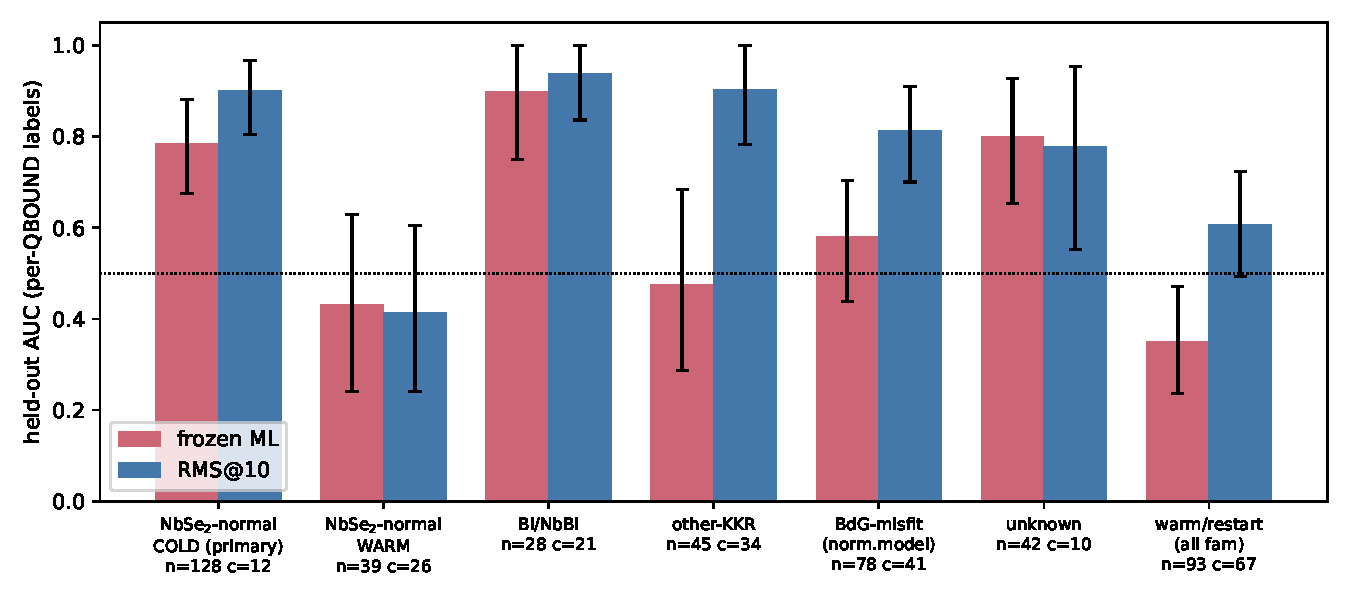
\includegraphics[width=0.85\textwidth]{figures/figD1_percohort.pdf}
\caption{Held-out per-cohort AUC (per-run \code{QBOUND} labels), frozen ML vs.\ RMS@10, with 95\% bootstrap
CIs. On the deployment target (NbSe$_2$-normal cold, leftmost) RMS@10 leads; the model is at or below
chance on other-material and warm/restart cohorts. There is no single pooled headline number.}
\label{fig:percohort}
\end{figure}

\paragraph{Scope consequences.} (i) BdG runs must be scored with the BdG model, not the normal one
(normal-model-on-BdG AUC $0.58$). (ii) Warm/restart runs are \emph{outside the current abort policy}: their
failures are rare and not separable from the early window (both methods $\approx$ chance), so they are
excluded from abort and left to run. (iii) No cross-material transfer is claimed for the learned model.

\section{The conformal early-abort policy}
\label{sec:conformal}
\paragraph{Guarantee.} Given a target $\alpha$, we abort a run iff its predicted convergence probability
is below a threshold calibrated on the campaign's converged runs. One-sided split conformal makes
\[
\Pr(\text{abort} \mid \text{the run would actually converge}) \le \alpha .
\]
Certifiability needs $\sim$19 calibration points at $\alpha=0.05$ ($\sim$9 at $0.10$); a campaign seeds
these from material-matched history and refreshes online. The guarantee holds under \emph{exchangeability}
of calibration and test runs; material-matched seeding plus online refresh is how we keep that assumption
approximately valid as a campaign drifts; a pre-registered violation trip-wire reverts to advisory mode
if the realized false-abort rate ever exceeds the budget.

\paragraph{The marginal-vs-conditional gap (found and fixed).} The split-conformal guarantee is
\emph{marginal}. Verified in out-of-sample replay: a single (marginal) threshold gives overall
false-abort $0.049$ at $\alpha=0.05$ but \textbf{0.086 conditional on the flat-starter stratum} --- the
very runs the dropped aligned window was meant to protect. The fix is \textbf{Mondrian
(group-conditional) thresholds}: one threshold per stratum (flat-starter vs.\ other, derived directly
from the feature vector, agreeing $100\%$ with the trajectory definition). This restores conditional
control to \textbf{0.047} (Fig.~\ref{fig:mondrian}, Table~\ref{tab:mondrian}). Both vehicles deploy Mondrian.

\begin{figure}[h]\centering
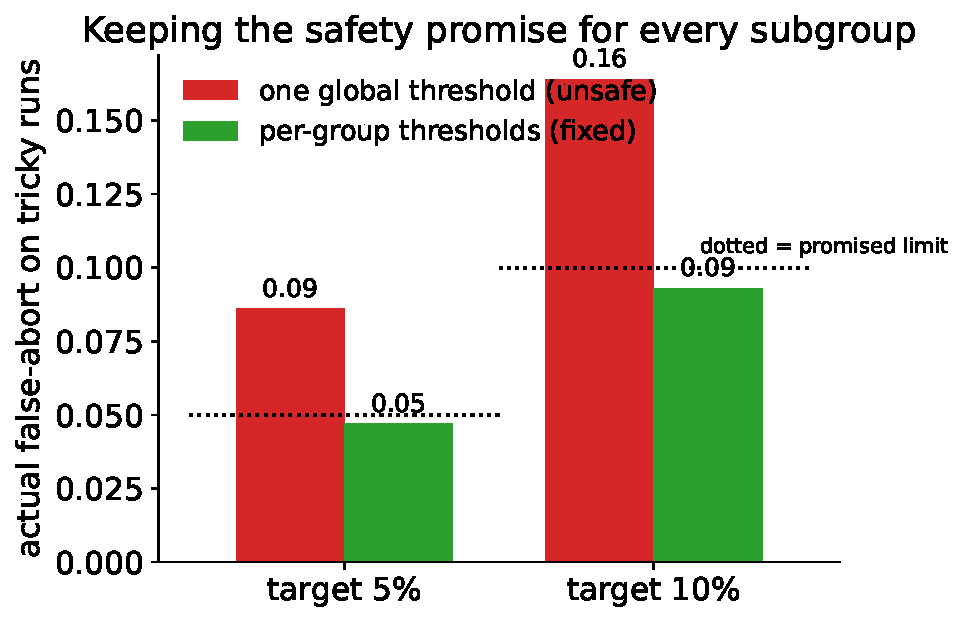
\includegraphics[width=0.55\textwidth]{figures/fig5_mondrian_safety.pdf}
\caption{The safety fix. A single global threshold breaks the false-abort promise on the tricky
``flat-start'' runs (red); one threshold per subgroup (green) restores the target rate within the
evaluated strata/cohort.}
\label{fig:mondrian}
\end{figure}

\paragraph{Seeded thresholds do not transport --- recalibrate per cohort.} The guarantee holds only under
\emph{exchangeability} of calibration and test runs, and the held-out data show this is not automatic. A
threshold seeded on historical NbSe$_2$ converged scores, applied to the broader held-out cohort, gave a
realized false-abort rate of \textbf{0.47} at $\alpha=0.10$ --- far above target: the seed does
\emph{not} transport across cohorts. The fix is \textbf{per-cohort recalibration}: re-deriving the
threshold on the deployment cohort's own converged runs restores realized false-abort to $\approx$ target
(0.10 $\to$ 0.098 for the model, 0.100 for RMS@10; Fig.~\ref{fig:transport}, nested-bootstrap
split-conformal, model weights frozen). The conformal guarantee is thus a \emph{per-cohort calibration}
property, not a transported one; deployment must recalibrate on the target cohort, and the trip-wire
reverts to advisory if the realized rate exceeds budget.

\begin{figure}[h]\centering
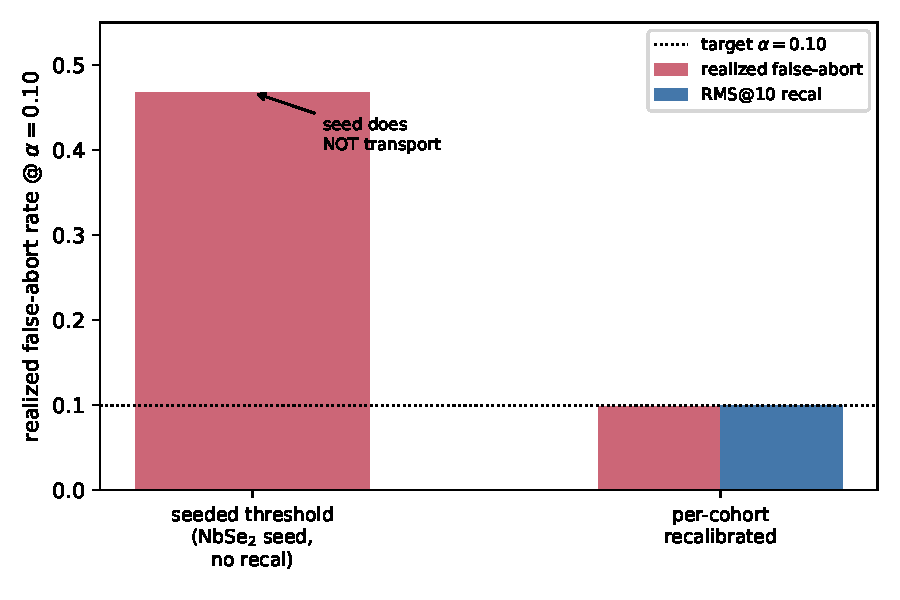
\includegraphics[width=0.5\textwidth]{figures/figD3_transport_recal.pdf}
\caption{The conformal threshold is a per-cohort object. A NbSe$_2$-seeded threshold applied to held-out
data breaks the false-abort promise (0.47 at $\alpha=0.10$); per-cohort recalibration (weights unchanged)
restores realized $\approx$ target for both the model and RMS@10.}
\label{fig:transport}
\end{figure}

\paragraph{Fallback discipline.} For BdG, if the $\Delta$ channel is unparseable the policy falls back to
an rms-only model \emph{with its own} conformal threshold (never comparing an rms-only score to an
rms+$\Delta$ threshold); both thresholds are certified independently.

\section{Deployment evaluation (per-cohort, calibrated)}
\label{sec:deploy}
All numbers are out-of-sample (Replay-OOF Invariant), accounted in SCF iterations (hardware-invariant),
and evaluated \emph{on the primary NbSe$_2$-normal cohort with per-cohort recalibration}
(Sec.~\ref{sec:heldout}). Each abort is charged at the deployment horizon (cumulative iteration 20, when
the model first scores under \code{nsteps}$=10$).

\paragraph{Recovery and false-abort, ML vs.\ RMS@10 (Fig.~\ref{fig:savings}, Table~\ref{tab:g1}).} With
per-cohort recalibration both policies hold realized false-abort at target ($\alpha=0.05/0.10/0.20 \to$
$0.04/0.10/0.20$). At matched $\alpha$ the \textbf{RMS@10 baseline recovers more wasted compute and catches
more doomed runs than the model}: failed-run recall $0.64/0.78/0.86$ (RMS@10) vs.\ $0.53/0.62/0.71$ (ML),
and fraction of wasted iterations saved $0.61/0.73/0.81$ vs.\ $0.54/0.62/0.69$. The model's abort precision
stays high ($\ge0.96$), but it is the weaker recovery policy on the primary cohort. This is the deployment
consequence of the held-out benchmark: \emph{a simple RMS@10 rule, per-cohort calibrated, is the stronger
early-abort policy here}.

\begin{figure}[h]\centering
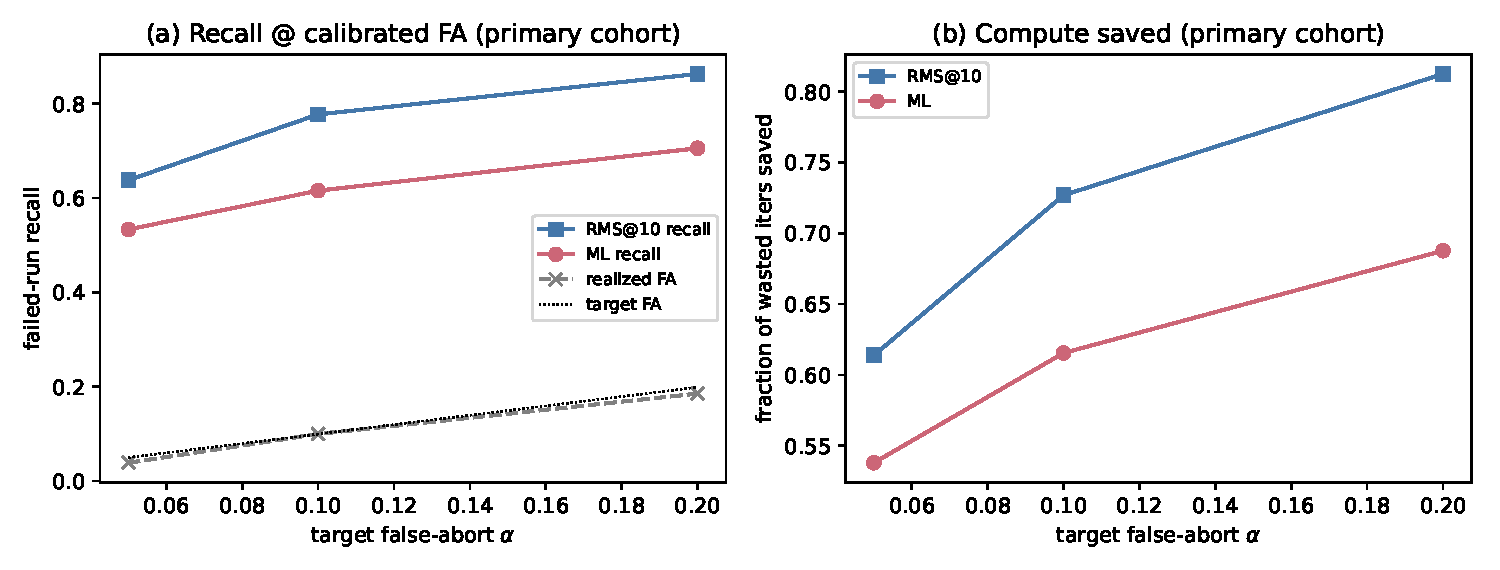
\includegraphics[width=0.92\textwidth]{figures/figD2_calibrated_savings.pdf}
\caption{Calibrated risk-savings on the primary NbSe$_2$-normal cohort (per-cohort recalibration, weights
frozen). (a) failed-run recall and (b) fraction of wasted iterations saved, both at matched realized
false-abort. RMS@10 (blue) dominates the frozen model (red) at every $\alpha$.}
\label{fig:savings}
\end{figure}

\paragraph{$\alpha$ economics.} Because a false abort under the auto-retry ladder \emph{warm-restarts}
(it does not discard a converging run), its cost is small, which pushes the net-optimal $\alpha$ upward.
The framework ships two profiles --- $\alpha=0.05$ (conservative) and $\alpha=0.10$ (throughput) --- but
the choice of \emph{scorer} (RMS@10 vs.\ model) is now itself a per-cohort decision, with RMS@10 the
default on the primary cohort.

\paragraph{The single-material prospective pilot (narrow).} An earlier prospective check calibrated on
329 historical NbSe$_2$ converged scores and applied to a held-out 2026 NbSe$_2$ grid (20 runs, verified
absent from training) gave a realized false-abort rate of $0.000$ at $\alpha=0.05$ and $0.10$. \textbf{This
is a narrow, single-material, in-distribution result} and must not be read as broad safety: the same seed,
applied to the wider held-out cohort, gave false-abort $0.47$ (Sec.~\ref{sec:conformal},
Fig.~\ref{fig:transport}). It demonstrates that \emph{material-matched} seeding worked on that single
2026 NbSe$_2$ grid, and reinforces the per-cohort-calibration requirement --- not cross-cohort transport.

\section{Live pilot: the abort machinery works end-to-end}
\label{sec:pilot}
Beyond retrospective replay, we ran the policy \emph{live} in the AiiDA daemon through a staged, gated
Fe-doped NbSe$_2$ pilot (Gate~0 $\to$ read-only pre-flight $\to$ advisory smokes $\to$ gated package
install/validation $\to$ stock baselines $\to$ ml\_assist arm). Five systems, each paired against a
matched stock counterfactual (same structure, cold start, mixing, segment cadence, partition). The pilot
validates the \emph{machinery}, not generalization; at $N{=}5$ every effect size is descriptive.

\begin{figure}[h]\centering
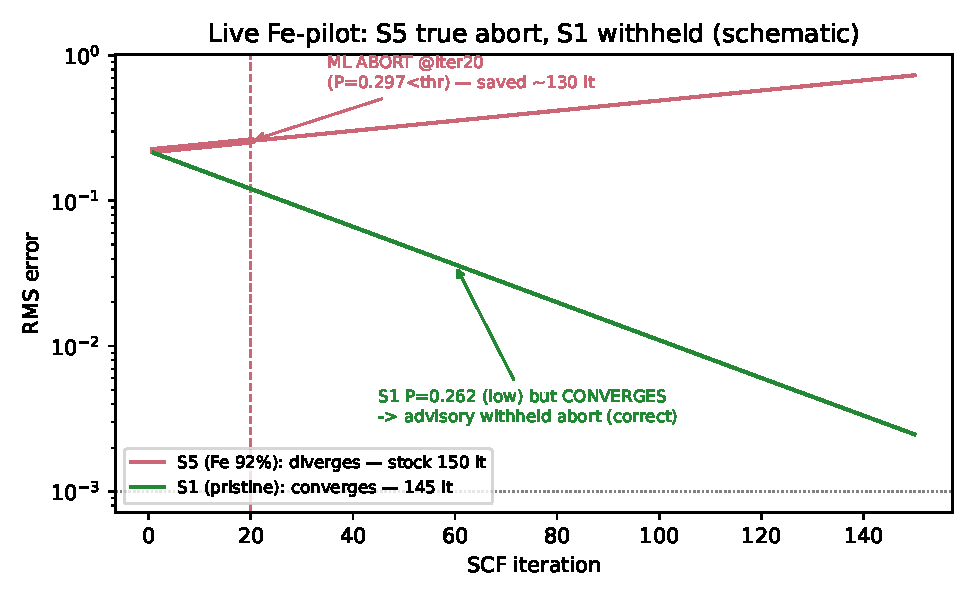
\includegraphics[width=0.62\textwidth]{figures/figD4_pilot.pdf}
\caption{Live pilot exemplars (schematic of recorded runs). \textbf{S5} (Fe~92\%) diverges; the frozen
model scored $P(\text{converge})=0.297$ below the abort threshold and issued a live \code{ERROR\_MLASSIST\_ABORT}
(exit 701) at cumulative iteration~20, saving $\approx$130 SCF iterations vs.\ its 150-iteration diverging
counterfactual. \textbf{S1} (pristine) scored low ($P=0.262$) yet converges; run advisory, its would-be
abort was correctly \emph{withheld} --- the deliberate conservative trade-off.}
\label{fig:pilot}
\end{figure}

\paragraph{What the pilot shows.} (i) A \textbf{true early abort} (S5) fired live end-to-end --- hook
$\to$ numpy inference $\to$ Mondrian per-stratum threshold $\to$ decision $\to$ telemetry $\to$ exit~701
--- and saved $\approx$130 iterations. (ii) A \textbf{would-be false abort was correctly withheld} (S1,
advisory), confirming the conservative-advisory default is the right guard for slowly-converging runs.
(iii) An \textbf{honest miss} (S3): a run whose stall emerges late was not caught by the early window ---
consistent with the held-out finding that late stalls are the hard case. The abort mechanism, telemetry,
and paired accounting are validated; the $N{=}5$ deltas are descriptive, not a powered savings claim.

\section{The BdG $\Delta$-channel}
\label{sec:delta}
The standard parser exposes RMS and charge-neutrality but not the pairing amplitude. We wrote a parser
for the \code{l-independent delta} lines KKRhost-BdG prints (two spin components per iteration, before
each iteration marker), yielding a per-iteration $\Delta$ trajectory (length verified equal to the
iteration count). Adding seven $\Delta$-shape features lifts within-BdG \emph{in-distribution} AUC from
\textbf{0.946 to 0.957} (95\% CI on the lift $[+0.000,+0.023]$; $\Delta$-only AUC $0.884$). (These are
in-distribution 5-fold numbers, like Table~\ref{tab:permaterial}, not held-out; and BdG runs must be
scored with this BdG model --- the normal model on BdG data reaches only AUC $0.58$,
Sec.~\ref{sec:heldout}.) The lift is modest here
because the historical corpus barely contains pairing-\emph{instability} runs (where $\Delta$ grows) ---
precisely the regime the parser targets for Vehicle A --- so it is expected to under-state the value on
the campaigns it is built for. The BdG model carries $\Delta$; every Vehicle-A run logs both the rms-only
and rms+$\Delta$ scores to measure the lift prospectively.

\section{Workflow hardening: four BdG footguns and the memory number}
\label{sec:footguns}
A separate but essential outcome: making \code{kkr\_bdg\_wc} run a multi-atom cell end-to-end. (Much
historical BdG ran instead as standalone \code{KkrCalculation}s in groups; the workchain is the path for
\emph{new} BdG runs, and the $\Delta$-parser of Sec.~\ref{sec:delta} works on any BdG \code{out\_kkr}
regardless of how it was launched.) Four
defaults, all tuned for a single-atom bulk reference, broke on an 8-atom NbSe$_2$ cell; each was fixed
and validated, and the fixes are folded into the workchain (v0.2.1--v0.2.4) and mirrored to the working
git branch:
\begin{enumerate}[leftmargin=1.6em,itemsep=1pt]
  \item \textbf{Multi-grid ranks.} MPI ranks must divide \emph{every} step's energy-point grid; a chain
  with a 24-point normal step and a 32-point BdG step requires a common divisor (or per-step ranks).
  \item \textbf{Cell-aware \code{RCLUSTZ}.} The screening-cluster radius now inherits the cell's value
  instead of a bulk default that overran the compiled cluster limit (\code{NACLSD}).
  \item \textbf{NSPIN-aware spin coupling.} BdG with \code{NSPIN=2} requires coupled spin channels; the
  workchain now drops the incompatible decoupling flag automatically.
  \item \textbf{Cell-aware \code{BZDIVIDE}.} The $k$-mesh inherits the cell's value; a bulk-dense mesh
  overran the compiled $k$-point limit (\code{KPOIBZ}) once BdG lowered the symmetry.
\end{enumerate}
With these fixed, an 8-atom BdG chain completed for the first time, giving the \textbf{Vehicle-A memory
number}: BdG job memory is \textbf{$\approx$1.0\,GB/rank}, \emph{flat with rank count} (energy-parallel
replication), i.e.\ $2.32\times$ the same-cell normal-state memory --- a mesh-robust scaling factor used
for cluster packing (Fig.~\ref{fig:memory}).

\begin{figure}[h]\centering
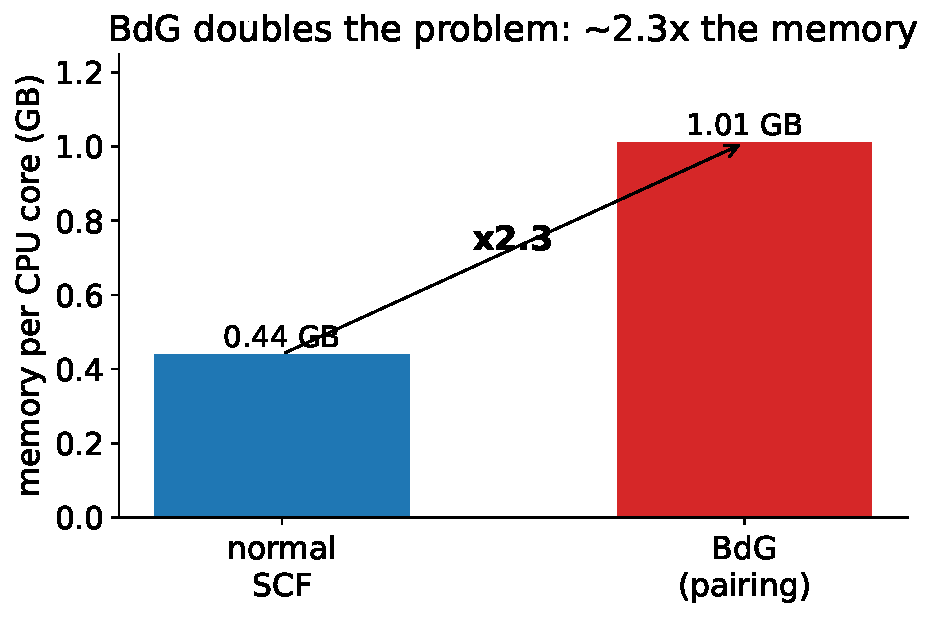
\includegraphics[width=0.5\textwidth]{figures/fig6_bdg_memory.pdf}
\caption{The BdG cost. Doubling the Hamiltonian into Nambu space raises memory per core by $\approx
2.3\times$; the factor is stable across core counts, which sets how many jobs fit on a node.}
\label{fig:memory}
\end{figure}

\section{Software package}
\label{sec:package}
Everything ships as an installable \code{aiida-kkr-mlassist} extension (src-layout), with the pure-numpy
core cleanly separated from the AiiDA workchain so inference needs no AiiDA and the daemon needs no
scikit-learn:
\begin{lstlisting}
aiida_kkr_mlassist/
  features.py    canonical 15-D feature schema (train == infer)
  infer.py       MLAssistModel  - numpy random forest (sklearn-exact)
  conformal.py   ConformalAbortPolicy + MondrianConformalAbortPolicy
  ranks.py       multi-step MPI-rank / energy-grid validator
  bdg_parser.py  BdG Delta-channel parser + features
  decision.py    config, decision state-machine, telemetry, graceful failure
  workchain.py   MLAssistKkrScfWorkChain  (entry point kkr.mlassist)
  models/        frozen artifacts + manifests + MODEL_CARD.md
\end{lstlisting}
The workchain is opt-in (an absent input reproduces stock behaviour) and records every decision in node
extras (advisory shadow data and audit trail). A unit-test suite (feature parity, golden parity, rank
validation, conformal shadow-replay, Mondrian control, decision state-machine, BdG parser, dual-scoring)
runs under the daemon interpreter to prove the deployment path is scikit-learn--free.

\section{Pre-registration and success gates (superseded)}
\label{sec:prereg}
Deployment was originally pre-registered as two campaigns (one shared preamble) with frozen model hashes,
the estimand definitions (\code{TOTAL\_CAMPAIGN\_ITER}, \code{MEDIAN\_ITER\_TO\_CONV}), an A/B fairness
rule (interleaved within a partition, wall-clock never pooled across partitions), a numeric
conformal-violation trip-wire, and a pre-commitment that failures are reported as-is. \textbf{This original
plan --- in particular the Vehicle-B throughput campaign and its \emph{G3} target --- was superseded} and
is retained here only for provenance:
\begin{description}[leftmargin=1.6em,itemsep=1pt]
  \item[Vehicle A (BdG, conservative).] rms+$\Delta$ model, dual-scoring telemetry, $\alpha=0.05$,
  Mondrian thresholds; a numeric near-criticality criterion controls how many cells are abort-enabled so
  the safety rule cannot silently starve the recovery gate; \emph{G2} target: recover $\ge50\%$ of the
  stock arm's own waste, zero conformal violations, physics-equality pass. \emph{(Not run --- BdG live
  campaign not launched.)}
  \item[Vehicle B (normal, throughput).] $\alpha=0.10$; \emph{paired within-system} A/B (Wilcoxon on
  iterations) for power; a paired warm-and-cold subset; an explicit racing ladder, commit rule, and
  warm-start donor-compatibility checks; \emph{G3} target: median iterations-to-converge and total campaign
  iterations both down $\ge25\%$.
\end{description}
\textbf{What actually happened.} The full Vehicle-B campaign was \emph{not} run: the planned dopant breadth
(Mn/V/Co) lived on the CLAIX cluster, which became unavailable, collapsing the design to an Fe-only iffslurm
pilot. That pilot ($N{=}5$, Sec.~\ref{sec:pilot}) validated the abort \emph{machinery} but is underpowered
for a Wilcoxon effect-size test, so \textbf{G3 is not an active claim}. The held-out benchmark
(Sec.~\ref{sec:heldout}) then reshaped the deployment recommendation itself: per-cohort calibration with an
RMS@10 comparator, rather than a fixed $\ge25\%$ throughput gate. Any future campaign must re-pre-register
against that recommendation.

\paragraph{Physics-equality tolerances (empirical).} Set from the intrinsic numerical reproducibility ---
the per-run total-energy variation over the last converged iterations (plateau noise, median
$1.6\times10^{-7}$\,Ry/atom over 2{,}833 runs). Between-run ``rerun'' scatter proved unusable
(formula-level matching still conflates dopant configurations). The adopted total-energy tolerance is
$3\times$ the plateau-noise 90th percentile, $\approx 3\times10^{-5}$\,Ry/atom --- neither contaminated
nor pathologically tight.

\section{Side studies and honest negatives}
\label{sec:negatives}
\begin{description}[leftmargin=1.6em,itemsep=1pt]
  \item[Impurity (KKRimp) feasibility.] Deferred: 2{,}390 impurity workchains exist, but their stored RMS
  trajectory has median length~1 --- per-iteration RMS is not in provenance --- so early-window prediction
  cannot be priced without richer logging. A logging change, not a modeling gap.
  \item[Warm-start (L3) matched pairs.] Underpowered: zero system-matched cold/warm converged pairs exist
  historically, so the causal warm-start effect is not retrospectively estimable and is deferred to the
  pre-registered randomized design.
\end{description}

\section{Reproducibility and governance}
\label{sec:governance}
The AiiDA database is treated read-only for analysis; any code-environment or database change is
confirmation-gated with a printed plan. Frozen models are versioned artifacts with SHA-256 and a manifest
recording feature schema, training-data hash, library versions, and out-of-sample AUC
(Appendix~\ref{app:prov}). The Replay-OOF Invariant, the two-denominator reporting rule, and the
negatives-are-publishable pre-commitment are the standing methodological safeguards.

\section{PotentialBank v1: L3 warm-start realized}
\label{sec:potbank}
The L3 lever --- reuse a converged potential instead of a cold Voronoi start --- is realized as
\textbf{PotentialBank~v1}: a provenance-clean catalog of certified single-structure converged KKR potentials,
each carrying a byte-exact compatibility fingerprint. A donor is admitted only if it passes \emph{E1
certification} verbatim: the parser succeeds and byte-exactly round-trips, the potential's per-type
$Z$-sequence matches the structure site order (empty spheres as $Z{=}0$), $\mathrm{NATYP}$ equals the site
count, the cell is non-CPA and non-BdG, NSPIN/SOC/LMAX/mesh parse, no mapping is guessed, and the staged,
AiiDA-retrieved, and manifest SHA-256 all agree. CPA, disordered, and BdG potentials are \emph{excluded by
construction}.

\paragraph{Coverage.} v1 contains \textbf{238 certified donor nodes = 237 unique-SHA donors} (one recorded
byte-duplicate: E1 Bi$_2$X$_4$ pk~24009$\equiv$24011), spanning \textbf{8 families, 35 materials, 42
compatibility classes}, of which \textbf{33 materials are F2-eligible} ($\ge 2$ independent certified donors):
NbSe$_2$/Bi (E1, 160 donors), simple metals Nb/Al/Cu/Ag/Mo (24), heavy-SOC Au/W/Pt/Sb/Pb (24), magnetic
Fe/Ni/Co (13), ordered intermetallics CuZn/Ni$_3$Al/FeAl (6), covalent empty-sphere Si/Ge (4), the metallic
layered chalcogenide TiSe$_2$ (2), and ionic rocksalt MgO/NaCl (4). Each family required its own certified
settings recipe (screening cluster RCLUSTZ, Chebyshev log panel R\_LOG/NPAN, BZ mesh, SOC key routing,
explicit empty-sphere mapping, and a mixing-path variation to obtain independent F2 pairs for deterministic
insulator SCF).

\paragraph{Warm-start savings (same-structure).} Injecting a certified donor as the start potential cuts
iterations-to-converge by large, reproducible margins, \emph{donor-choice-independent} (33/33 targets:
identical iterations from either donor) and direction-symmetric where cold-comparable:
\begin{center}\small
\begin{tabular}{lccc}
\toprule
family & cold iters & warm iters & \% saved \\
\midrule
simple metals & 66--102 & 4--7 & 91--94\,\% \\
heavy-SOC & 122--136 & 2--3 & $\sim$97\,\% \\
magnetic & 131--136 & 5--6 & $\sim$96\,\% \\
covalent Si/Ge & 117--119 & 2--3 & 97--98\,\% \\
intermetallics & 128--152 & 5--7 & 95--97\,\% \\
TiSe$_2$ (layered) & 1188--1354 & $\le$100 & $\sim$92\,\% \\
ionic MgO/NaCl & 171--750 & 2--500 & 33--99\,\% \\
\bottomrule
\end{tabular}
\end{center}
The magnitude is set by the target's mixing accelerator (a Broyden target polishes a warm start in a few
iterations; a pure-linear target still crawls, e.g.\ 500 vs.\ 750 for MgO/NaCl), so each row is a
\emph{matched same-mixing} warm-vs-cold comparison and we report per-family, never a single pooled headline.
Contour caveats are recorded (TiSe$_2$ is coarse-converged only, as the fine contour destabilizes the
zero-gap semimetal). Coverage, F2-eligibility, warm-vs-cold, savings distribution, the parked-hard-case map,
and the provenance workflow are in Figs.~1--6 of the v1 synthesis package.

\paragraph{Limitations.} PotentialBank v1 supports \textbf{same-structure reuse only}; it is \emph{not} a
cross-material transfer claim and \emph{not} a guaranteed acceleration (donor$\equiv$target geometry,
chemistry, and settings; savings depend on structure/mixing/contour). CPA/doped/disordered and BdG are out of
scope. Nine hard cases are parked with root causes (MoS$_2$ and NbS$_2$ NACLSD, WSe$_2$ SOC contour/EMIN
instability, TaS$_2$ SOC-NaN, TiAl VERTEX3D, Bi$_2$Te$_3$/Bi$_2$Se$_3$ hard-convergence, CaF$_2$/LiF). The
warm-start outputs are benchmarks and are \emph{not} themselves certified as donors. For \code{ml\_assist}, the
early-abort mechanism is validated live but broad ML transfer is \emph{not} proven --- it does not beat a
simple RMS@10 baseline out-of-sample and requires per-cohort recalibration.

\subsection{Related work}
\label{sec:relatedwork}
\textbf{Workflow and provenance.} We build directly on AiiDA-KKR\,/\,JuKKR~\cite{aiidakkr}, which provide the
KKR restart and \code{potential\_overwrite} primitives our warm start uses. aiida-mlip~\cite{aiidamlip} is a
sibling AiiDA plugin that applies the same provenance discipline to machine-learned interatomic potentials, a
different target. \textbf{Predicting quantities to accelerate SCF.} A growing body of work \emph{predicts} an
electronic-structure quantity to speed up or bypass self-consistency: ChargE3Net~\cite{charge3net} predicts the
charge density and reports a $26.7\%$ reduction in SCF iterations when initializing DFT on \emph{unseen}
materials; SALTED~\cite{salted} learns 3D electron densities via density fitting; and
DeepH\,/\,DeepH-E3~\cite{deeph,deephe3} predict the DFT Hamiltonian directly. mp-pyrho~\cite{pyrho} provides
representation-independent charge-density regridding and an associated density database. \textbf{Representations
and MLIP tooling.} DScribe~\cite{dscribe} supplies atomistic descriptors; DP-GEN~\cite{dpgen} performs
concurrent-learning generation of deep-potential models; dftio~\cite{dftio} standardizes DFT outputs for machine
learning. \textbf{Where we differ.} These methods \emph{learn to predict} a density, potential, or Hamiltonian
and, in the best cases, transfer across chemistries. PotentialBank v1 makes \textbf{no prediction and no
cross-material claim}: it \emph{reuses an existing, certified potential for the identical structure}. The
novelty is the certification and retrieval policy --- integrity, compatibility, scope, and auditability --- not
a new physical model or a learned mapping. We are not aware of a verified KKR-specific tool that provides this
certified same-structure reuse layer.

\paragraph{What is and is not novel.} We do \textbf{not} claim to have invented KKR restart, potential
overwriting, or SCF warm starting --- those primitives exist in AiiDA-KKR and are standard practice. We do
\textbf{not} predict potentials, densities, or Hamiltonians, and we make no cross-material transfer claim. What
is novel is the \textbf{provenance-certified reuse layer}: automated donor discovery over the provenance graph;
a strict, auditable eligibility policy (byte-exact integrity, exact structural compatibility, non-CPA\,/\,non-BdG
scope, no guessed mapping); an optional convergence advisor with explicitly benchmarked limits; and honest
same-structure warm-start benchmarks together with a documented catalog of hard cases and negative results.

\section{Status and roadmap}
\label{sec:status}
\textbf{Complete and validated:} the framework and its pure-numpy artifact; the conformal (Mondrian)
abort policy; the live pilot (abort mechanism validated end-to-end, Sec.~\ref{sec:pilot}); the
leakage-clean held-out benchmark (Sec.~\ref{sec:heldout}); the BdG $\Delta$-parser and frozen BdG models;
the \code{aiida-kkr-mlassist} package with tests; the BdG workchain hardening and memory number; the
physics-equality tolerance; the pre-registrations.
\textbf{Key finding for deployment:} the learned model does not beat a simple RMS@10 rule out-of-sample on
the primary cohort, does not transfer across materials, and its conformal guarantee requires
\emph{per-cohort recalibration}. Deployment is therefore per-cohort and baseline-benchmarked: the default
scorer on the primary cohort is RMS@10, and any campaign must recalibrate the abort threshold on its own
converged runs and compare model vs.\ RMS@10 before enabling abort.
\textbf{Remaining modeling gap:} late-stall detection (largely missed by the early window, for both the
model and RMS@10). \textbf{L3 (warm start) is delivered} as PotentialBank~v1 (Sec.~\ref{sec:potbank}): 237
certified single-structure donors across 8 families with measured same-structure savings; \textbf{L2}
(mixing search) remains estimated by the pre-registered campaigns. PotentialBank~v1 is same-structure reuse
only --- no cross-material transfer, no guaranteed acceleration.

\section{Software and data availability}
\label{sec:availability}
The software is open source under the \textbf{MIT} license and is available at
\texttt{https://github.com/MRHemmati/kkr\_ml\_tools} (a tagged release and archival DOI will be minted on
acceptance and recorded here). The repository ships the installable \code{aiida-kkr-mlassist} package and the
\code{kkr\_convergence\_advisor}, unit tests, the frozen model artifacts with SHA-256 manifests, the
PotentialBank~v1 manifest\,/\,tables\,/\,figures, the advisor index, and two walkthrough notebooks. \textbf{Data
availability:} the derived artifacts (manifests, benchmark tables, model manifests) are included; the raw KKR
potential files are \emph{not} redistributed --- they remain in the AiiDA provenance store and are referenced by
byte-exact SHA-256 and provenance handles (\code{seg\_pk}, \code{wc\_pk}, \code{uuid}), so their identity is
verifiable by anyone with access to that store. Live KKR submissions require the JuKKR codes and the authors'
AiiDA database and cluster environment.
\emph{Versioning:} the Python \emph{package} (\code{aiida-kkr-mlassist}) and the \emph{data release}
(PotentialBank and advisor index) are versioned independently --- the package is at \code{0.1.1}, while the
certified potential catalog and advisor index are the frozen \emph{PotentialBank~v1} release; these are distinct
artifacts and the different version labels are intentional, not an inconsistency.

\section{Reproducibility}
\label{sec:reproducibility}
Offline, without HPC or AiiDA: install from source (\code{pip install -e .}, \code{numpy}-only core), load the
advisor index (\code{kkr\_convergence\_advisor.load\_index()}), run the self-asserting unit tests
(\code{PYTHONPATH=src python tests/*.py}), and execute the two walkthrough notebooks (the submission tutorial is
safe-by-default and submits nothing). A lightweight smoke test reproduces the headline counts
($237/238/8/33$); \code{sha256sum -c reports/potentialbank\_v1/MANIFEST.sha256} verifies the synthesis bundle.
The reviewer-run checklist gives exact commands and expected outputs.

\section*{CRediT author contribution statement}
\emph{TODO before submission: complete CRediT roles per author (e.g.\ Conceptualization, Methodology, Software,
Validation, Investigation, Data curation, Writing --- original draft, Writing --- review \& editing).}

\section*{Declaration of competing interest}
The authors declare that they have no known competing financial interests or personal relationships that could
have appeared to influence the work reported in this paper.

\section*{Acknowledgments}
\emph{TODO: funding sources, computing allocations (iffslurm), and collaborators.}

\section*{Use of AI assistance}
AI coding and writing assistants were used to help draft text, generate code-edit suggestions, and organize
reports; all scientific decisions, calculations, validation, and final claims were reviewed by the author.

\appendix
\section{Result tables}
\label{app:tables}

\begin{table}[h]\centering
\caption{Per-material convergence AUC, \emph{in-distribution} 5-fold cross-validation (deduplicated runs).
Strong where data is plentiful; honestly weaker/underpowered where thin. \textbf{These are same-distribution
CV numbers, not the deployment metric} --- for the leakage-clean held-out result see
Table~\ref{tab:percohort}. No cross-material transfer is claimed.}
\label{tab:permaterial}
\begin{tabular}{lccc}
\toprule
family & $n$ & OOF AUC & 95\% CI \\
\midrule
NbSe$_2$        & 373  & 0.918 & [0.86, 0.97] \\
Bi/NbBi         & 38   & 0.849 & [0.69, 0.97] \\
mixed/unknown\footnotemark & 1398 & 0.950 & [0.92, 0.97] \\
\midrule
pooled (normal, frozen model) & 1830 & 0.944\footnotemark[3] & --- \\
\bottomrule
\end{tabular}
\end{table}
\footnotetext[3]{In-distribution 5-fold CV; \emph{not} the deployment headline. Out-of-sample on the
primary NbSe$_2$-normal cohort the frozen model reaches AUC $0.83$ and is beaten by RMS@10 $0.90$
(Table~\ref{tab:percohort}).}
\footnotetext{``mixed/unknown'' = runs whose chemical formula could not be recovered from provenance and
so could not be assigned to the NbSe$_2$ or Bi/NbBi families; they are the largest, cleanest group and
anchor the pooled model.}

\begin{table}[h]\centering
\caption{The ML margin over baselines, \emph{in-distribution only}. Out-of-sample the relevant baseline is
RMS@10 (not the weak extrapolation heuristic), and it matches or beats the model per cohort
(Table~\ref{tab:percohort}).}
\label{tab:baselines}
\begin{tabular}{lcc}
\toprule
method & in-distribution AUC & held-out (primary cohort) AUC \\
\midrule
physical extrapolation heuristic & 0.549 & --- \\
logistic regression              & 0.826 & --- \\
RMS@10 rule (simple baseline)    & --- & \textbf{0.897} \\
random forest (\code{ml\_assist})& \textbf{0.944} & 0.831 \\
\bottomrule
\end{tabular}
\end{table}

\begin{table}[h]\centering
\caption{Marginal vs.\ Mondrian conformal, false-abort rate (out-of-sample). The marginal threshold
under-protects the flat-starter stratum; per-stratum (Mondrian) thresholds restore conditional control.}
\label{tab:mondrian}
\begin{tabular}{lccc}
\toprule
$\alpha$ & marginal (overall) & marginal (flat-starters) & Mondrian (flat-starters) \\
\midrule
0.05 & 0.049 & 0.086 & \textbf{0.047} \\
0.10 & 0.098 & 0.164 & \textbf{0.093} \\
\bottomrule
\end{tabular}
\end{table}

\begin{table}[h]\centering
\caption{Calibrated early-abort on the primary NbSe$_2$-normal cohort (held-out, per-cohort
recalibration, weights frozen; nested-bootstrap split-conformal, iterations). Realized false-abort holds
at target for both; \textbf{RMS@10 recovers more and catches more doomed runs than the model at every
$\alpha$}.}
\label{tab:g1}
\begin{tabular}{lcccc}
\toprule
$\alpha$ & policy & realized false-abort & failed-run recall & wasted-iters saved \\
\midrule
0.05 & frozen ML & 0.036 & 0.53 & 0.54 \\
0.05 & RMS@10    & 0.039 & \textbf{0.64} & \textbf{0.61} \\
0.10 & frozen ML & 0.096 & 0.62 & 0.62 \\
0.10 & RMS@10    & 0.100 & \textbf{0.78} & \textbf{0.73} \\
0.20 & frozen ML & 0.196 & 0.71 & 0.69 \\
0.20 & RMS@10    & 0.186 & \textbf{0.86} & \textbf{0.81} \\
\bottomrule
\end{tabular}
\end{table}

\section{Model provenance}
\label{app:prov}
Frozen artifacts (pure-numpy, golden-parity $=0$ vs.\ scikit-learn, versioned by SHA-256):
\begin{center}
\begin{tabular}{llcc}
\toprule
model & role & features & in-dist.\ AUC\footnotemark[4] \\
\midrule
\code{mlassist\_v1\_normal\_fixed10} & normal-state & 15 & 0.944 \\
\code{mlassist\_v1\_bdg\_rmsdelta}   & BdG primary  & 22 & 0.957 \\
\code{mlassist\_v1\_bdg\_rms}        & BdG missing-$\Delta$ fallback & 15 & 0.946 \\
\bottomrule
\end{tabular}
\footnotetext[4]{In-distribution 5-fold CV. Held-out, the normal model scores $0.83$ on its primary cohort
(Table~\ref{tab:percohort}); weights were unchanged through all held-out and pilot evaluations.}
\end{center}
Each artifact ships a JSON manifest (feature names, training-data SHA-256, library versions, creation
timestamp, golden-parity value) and a model card stating intended use, per-system scope, and the
Replay-OOF Invariant.

\begin{thebibliography}{99}
\bibitem{aiidakkr} P.~R\"u{\ss}mann, F.~Bertoldo, and S.~Bl\"ugel, ``The AiiDA-KKR plugin and its application to
  high-throughput impurity embedding into a topological insulator,'' \emph{npj Comput.\ Mater.} \textbf{7}, 13
  (2021), DOI 10.1038/s41524-020-00482-5. Software (JuKKR): \texttt{https://github.com/JuDFTteam/aiida-kkr};
  docs \texttt{https://aiida-kkr.readthedocs.io} (User guide: Calculations, Workflows).
\bibitem{aiidamlip} STFC, \emph{aiida-mlip: machine-learned interatomic potentials in AiiDA} (software
  documentation, BSD-3). \texttt{https://github.com/stfc/aiida-mlip}; docs
  \texttt{https://stfc.github.io/aiida-mlip/}.
\bibitem{dscribe} L.~Himanen \emph{et al.}, ``DScribe: Library of descriptors for machine learning in materials
  science,'' \emph{Comput.\ Phys.\ Commun.} \textbf{247}, 106949 (2020); arXiv:1904.08875.
\bibitem{dpgen} Y.~Zhang \emph{et al.}, ``DP-GEN: A concurrent learning platform for the generation of reliable
  deep learning based potential energy models,'' \emph{Comput.\ Phys.\ Commun.} \textbf{253}, 107206 (2020);
  arXiv:1910.12690.
\bibitem{dftio} DeePModeling community, \emph{dftio: transcribing DFT outputs into ML-ready formats} (software
  documentation, MIT). \texttt{https://github.com/deepmodeling/dftio}; docs
  \texttt{https://deepmodeling.github.io/dftio/}.
\bibitem{pyrho} J.~Shen \emph{et al.}, ``A representation-independent electronic charge density database for
  crystalline materials,'' \emph{Sci.\ Data} \textbf{9}, 661 (2022); arXiv:2107.03540. Software:
  \texttt{https://github.com/materialsproject/pyrho}.
\bibitem{charge3net} T.~Koker \emph{et al.}, ``Higher-order equivariant neural networks for charge density
  prediction in materials,'' \emph{npj Comput.\ Mater.} \textbf{10}, 138 (2024); arXiv:2312.05388.
\bibitem{salted} A.~M.~Lewis, A.~Grisafi, M.~Ceriotti, and M.~Rossi, ``Learning electron densities in the
  condensed phase'' (SALTED), \emph{J.\ Chem.\ Theory Comput.} \textbf{17}, 7203 (2021), DOI
  10.1021/acs.jctc.1c00576; arXiv:2106.05364. Docs \texttt{https://salted.readthedocs.io}.
\bibitem{deeph} H.~Li \emph{et al.}, ``Deep-learning density functional theory Hamiltonian for efficient ab
  initio electronic-structure calculation,'' \emph{Nat.\ Comput.\ Sci.} \textbf{2}, 367 (2022).
\bibitem{deephe3} X.~Gong \emph{et al.}, ``General framework for E(3)-equivariant neural network representation
  of density functional theory Hamiltonian'' (DeepH-E3), \emph{Nat.\ Commun.} \textbf{14}, 2848 (2023).
\end{thebibliography}

\end{document}
